% Exam Template for UMTYMP and Math Department courses
%
% Using Philip Hirschhorn's exam.cls: http://www-math.mit.edu/~psh/#ExamCls
%
% run pdflatex on a finished exam at least three times to do the grading table on front page.
%
%%%%%%%%%%%%%%%%%%%%%%%%%%%%%%%%%%%%%%%%%%%%%%%%%%%%%%%%%%%%%%%%%%%%%%%%%%%%%%%%%%%%%%%%%%%%%%

% These lines can probably stay unchanged, although you can remove the last
% two packages if you're not making pictures with tikz.
\documentclass[11pt]{exam}
\RequirePackage{amssymb, amsfonts, amsmath, latexsym, xspace, setspace}
\RequirePackage{tikz, pgflibraryplotmarks}

% By default LaTeX uses large margins.  This doesn't work well on exams; problems
% end up in the "middle" of the page, reducing the amount of space for students
% to work on them.
\usepackage[margin=1in]{geometry}
\usepackage{verbatim}

% Here's where you edit the Class, Exam, Date, etc.
\newcommand{\class}{Principles of Operating Systems}
\newcommand{\term}{Fall 2018}
\newcommand{\examnum}{Final}
\newcommand{\examdate}{12/13/2018}
\newcommand{\timelimit}{1:30pm -- 3:30pm}

% For an exam, single spacing is most appropriate
\singlespacing
% \onehalfspacing
% \doublespacing

% For an exam, we generally want to turn off paragraph indentation
\parindent 0ex

\def\answers{1}


\begin{document} 

% These commands set up the running header on the top of the exam pages
\pagestyle{head}
\firstpageheader{}{}{}
\runningheader{\class}{\examnum\ - Page \thepage\ of
\numpages}{\fbox{\rule{2in}{0pt}\rule[-0.5ex]{0pt}{5ex}}}
\runningheadrule

\begin{flushright}
\begin{tabular}{p{2.8in} r l}
%\textbf{\class} & \textbf{Name (Print):} & \makebox[2in]{\hrulefill}\\
  \textbf{\class} & \textbf{Name (Print):} &
  \fbox{\rule{2in}{0pt}\rule[-0.5ex]{0pt}{5ex}}\\
\textbf{\term} &&\\
\textbf{\examnum} &&\\
\textbf{\examdate} &&\\
\textbf{Time Limit: \timelimit} & & \\
\end{tabular}\\
\end{flushright}
\rule[1ex]{\textwidth}{.1pt}




%\begin{minipage}[t]{3.7in}
%\vspace{0pt}
\begin{itemize}

\item \textbf{Don't forget to write your name on this exam.} 

\item \textbf{This is an open book, open notes exam. But no online or 
    in-class chatting.  } 

    
\item \textbf{Ask us if something is confusing.}

\item \textbf{Organize your work}, in a reasonably neat and coherent way, in
the space provided. Work scattered all over the page without a clear ordering will 
receive very little credit.  

\item \textbf{Mysterious or unsupported answers will not receive full
credit}.  A correct answer, unsupported by explanation will receive no credit; 
an incorrect answer supported by substantially correct explanations might still 
receive partial credit.

\item If you need more space, use the back of the pages; clearly indicate when you have done this.

\item \textbf{Don't forget to write your name on this exam.} 


\end{itemize}

%Do not write in the table to the right.
%\end{minipage}
%\hfill

%\begin{minipage}[t]{2.3in}
%\vspace{0pt}
%\cellwidth{3em}
%\gradetablestretch{2}
\vqword{Problem}
\addpoints % required here by exam.cls, even though questions haven't started yet.	
\gradetable[v]%[pages]  % Use [pages] to have grading table by page instead of question

%\end{minipage}
\newpage % End of cover page

%%%%%%%%%%%%%%%%%%%%%%%%%%%%%%%%%%%%%%%%%%%%%%%%%%%%%%%%%%%%%%%%%%%%%%%%%%%%%%%%%%%%%
%
% See http://www-math.mit.edu/~psh/#ExamCls for full documentation, but the questions
% below give an idea of how to write questions [with parts] and have the points
% tracked automatically on the cover page.
%
%
%%%%%%%%%%%%%%%%%%%%%%%%%%%%%%%%%%%%%%%%%%%%%%%%%%%%%%%%%%%%%%%%%%%%%%%%%%%%%%%%%%%%%

\begin{questions}

\addpoints 
\question Pipes

Xv6 shell implements a pipe command (e.g., \texttt{ls | wc}) with the following code: 

\begin{verbatim}
8650   case PIPE:
8651     pcmd = (struct pipecmd*)cmd;
8652     if(pipe(p) < 0)
8653       panic("pipe");
         // Point A
8654     if(fork1() == 0){
8655       close(1);
8656       dup(p[1]);
8657       close(p[0]);
8658       close(p[1]);
           // point B
8659       runcmd(pcmd->left);
8660     }
8661     if(fork1() == 0){
8662       close(0);
8663       dup(p[0]);
8664       close(p[0]);
8665       close(p[1]);
8666       runcmd(pcmd->right);
8667     }
8668     close(p[0]);
8669     close(p[1]);
         // point C
8670     wait();
8671     wait();
8672     break
\end{verbatim}

Draw the connections between file descriptors, I/O devices and pipes at points
A, B above.  Connections can be depicted with lines with arrows. The error is
aligned with the direction of data flow, i.e., if the file is written the error
points at the file object. 

Hint: pay attention to close() dup() calls before and after the point


\begin{parts}

\newpage

\part[5] Point A

\begin{figure}[h] 
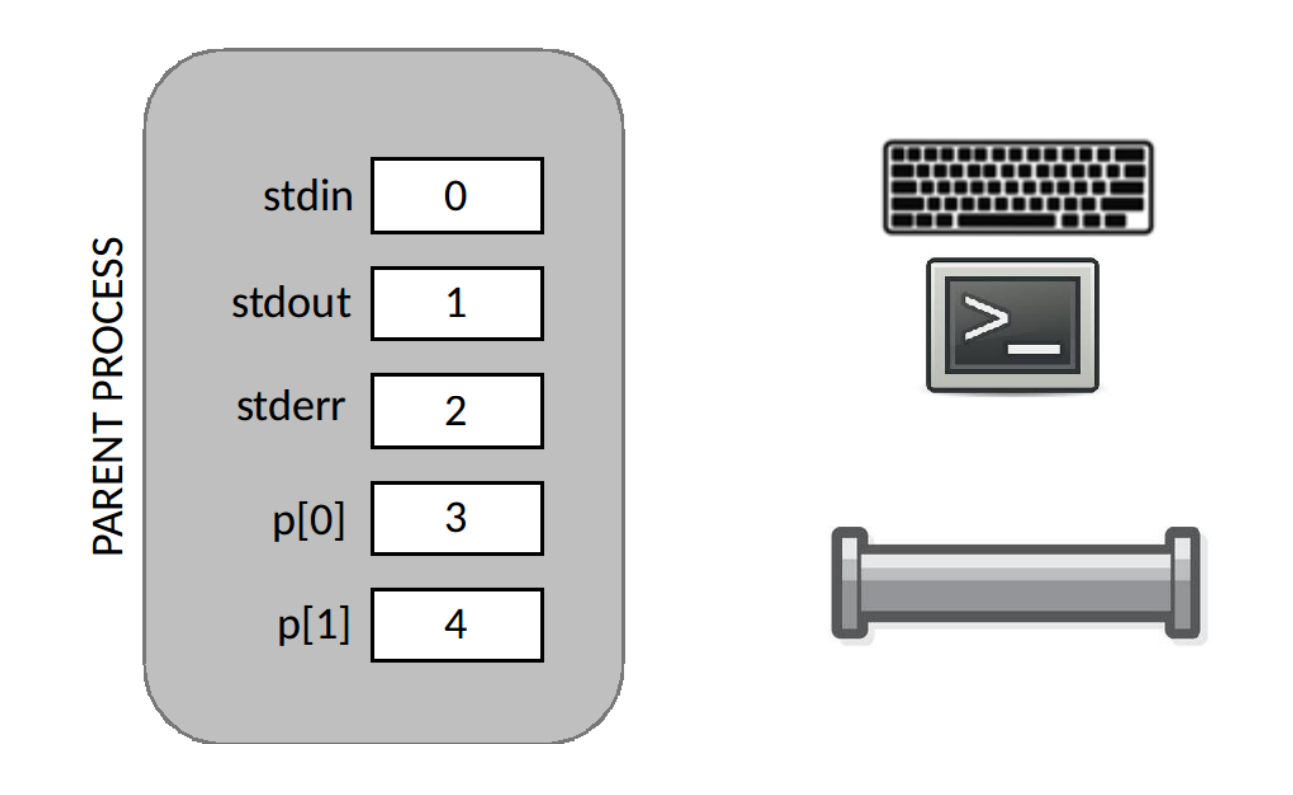
\includegraphics[width=0.5\columnwidth]{figs/point-a-temp}
\label{fig:point-a}
\end{figure}

\part[5] Point B

\begin{figure}[h] 
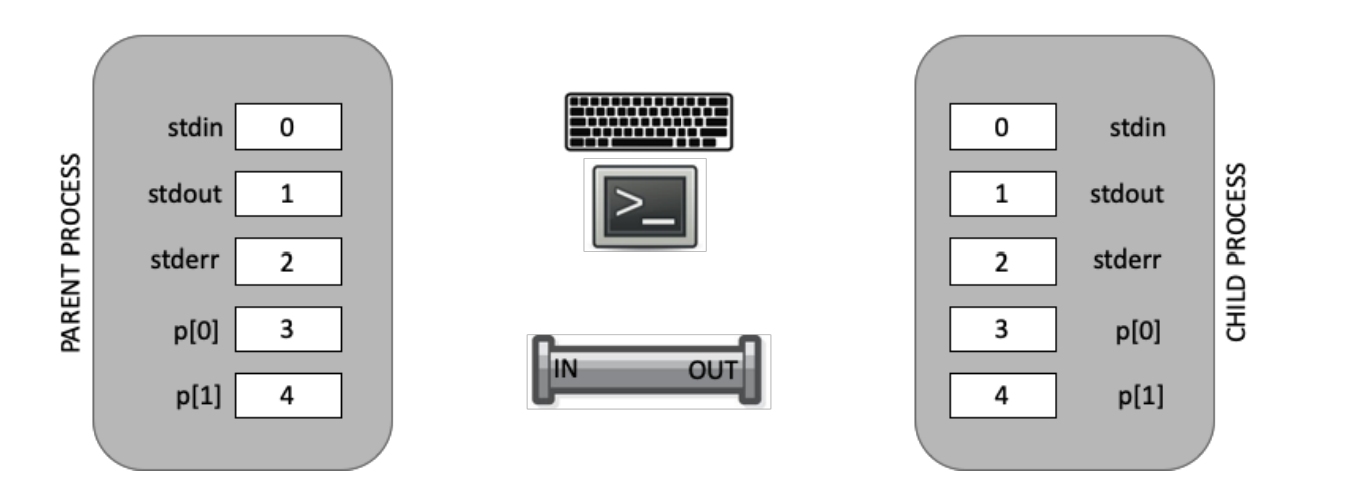
\includegraphics[width=0.8\columnwidth]{figs/point-b-temp}
\label{fig:point-b}
\end{figure}


\newpage

\part[5] Point C

\begin{figure}[h] 
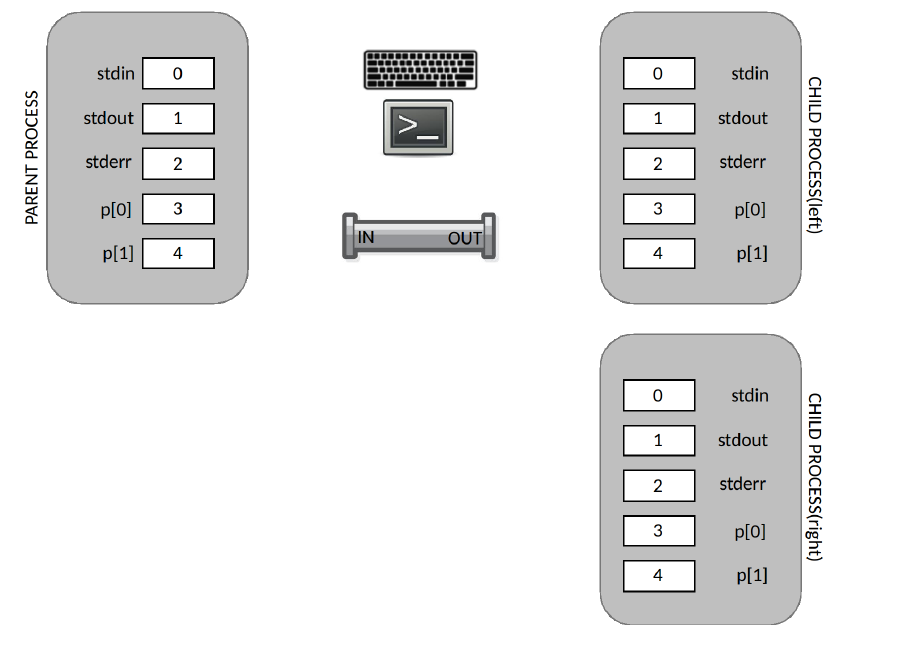
\includegraphics[width=0.8\columnwidth]{figs/point-c-temp}
\label{fig:point-c}
\end{figure}





\end{parts}


\addpoints 
\question Processes and system calls

\begin{parts}

\part[5] What is the first system call executed by xv6? Explain your answer. 
\vfill

\end{parts}


\newpage

\addpoints
\question Interrupts and context switch

\begin{parts} 

\part[5] When a user-program (a program that executes at current privilege
level 3) is preempted with an interrupt five registers are saved by the
hardware: ESP, SS, EFLAGS, CS, EIP. Why these five registers have to be saved,
but others, e.g., EAX, ECX, etc., don't? 
\vfill 


\part[5] During the context switch the code of the \texttt{swtch()} function
visibly does not save the EIP register. How is it saved and restored then
during the context switch?  
\vfill 

\newpage

\part[5] The \texttt{fork()} system call returns ``0'' inside the child
process. This return value is passed to the child process from inside the
\texttt{fork()} system call with the following line: 

\begin{verbatim} 
np->tf->eax = 0 
\end{verbatim}

Explain how does this work, i.e., how the ``0'' value ends up being 
returned by the fork() inside the user process. 
\vfill 

\part[5] What does the stack look inside the \texttt{bar()} function. Draw a diagram, provide a short description for every value on the stack. 

\begin{verbatim}
int bar(int a, void *buffer, int size) {


}; 
\end{verbatim} 
\vfill 

\iffalse

\part[5] Buffer overflow is an attack that redirects control flow ... 
\vfill 

\fi


\end{parts}

\newpage

% Basic question
\addpoints \question File system


Xv6 lays out the file system on disk as follows:

\begin{figure}[h] \centering
  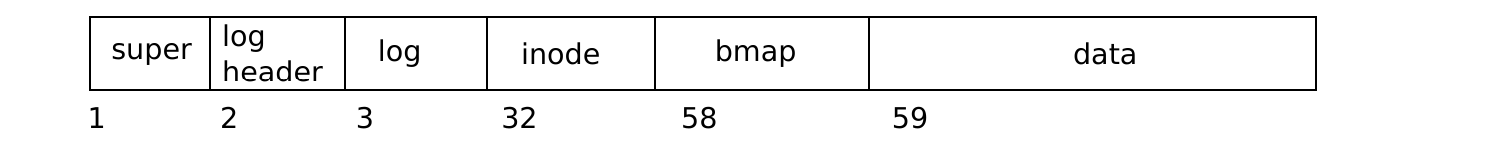
\includegraphics[width=0.8\columnwidth]{figs/fs}
  \label{fig:ramengine-decomposed-app}

\end{figure}

Block 1 contains the super block. Blocks 2 through 31 contain the log header
and the log. Blocks 32 through 57 contain inodes. Block 58 contains the bitmap
of free blocks. Blocks 59 through the end of the disk contain data blocks. 

 
\begin{parts} 

\part[5] Every file system transaction that changes the file system write one 
disk block twice. What is this block (what's its block number) and why is it 
written twice? 
\vfill 

\end{parts}

\newpage
\addpoints
\question Synchronization

\begin{parts}

\part[5] Sleep  has  to  check \texttt{lk != \&ptable.lock} to  avoid a deadlock.  Suppose the
special  case when the following lines 

\begin{verbatim}
if(lk != &ptable.lock) { 
  acquire(&ptable.lock);
  release(lk);
}
\end{verbatim}

are replaced with

\begin{verbatim}
release(lk);
acquire(&ptable.lock);
\end{verbatim}

Doing this would break sleep. How?
\vfill

\part[5] Now Alice decides to put the following code instead of the original \texttt{xchg()} loop in the \texttt{acquire()} function 

\begin{verbatim}
for(;;) {
  if(!lk->locked)
  {
    lk->locked = 1;
    break;
  }
}
\end{verbatim}

She boots xv6 on a multi-processor machine, explain what happens?
\vfill 

\end{parts}

\newpage
\addpoints

\question cs143A. I would like to hear your opinions about cs143A, so please answer the following questions. (Any answer, except
no answer, will receive full credit.)


\begin{parts}

\part[1] Grade cs143A on a scale of 0 (worst) to 10 (best)?

\vfill

\part[2] Any suggestions for how to improve cs143A?

\vfill

\part[1] What is the best aspect of cs143A?

\vfill

\part[1] What is the worst aspect of cs143A?

\vfill

\end{parts}


% If you want the total number of points for a question displayed at the top,
% as well as the number of points for each part, then you must turn off the point-counter
% or they will be double counted.
%\newpage
%\addpoints
%\question[10] Even more work.
%\noaddpoints % If you remove this line, the grading table will show 20 points 
%for this problem.
%\begin{parts} \part[5] Even more...  \vspace{4.5in} \part[5] That's clearly
%too much \end{parts}



\end{questions}
\end{document}
